% 编译方式: latexmk -xelatex 或 xelatex -> bibtex -> xelatex*2
\documentclass{ctexart}
\usepackage{amsmath} % 数学符号 & 方程
\usepackage{amssymb} % 特殊数学符号
\usepackage{graphicx} % 图形 & 图像
\usepackage{hyperref} % 超链接
\usepackage{syntonly} % 仅语法检查
\usepackage{textcomp} % 特殊符号
\usepackage{ulem} % 内容强调
\usepackage{verbatim} % 长注释
%\syntaxonly
\hyphenation{}
\normalem
\hypersetup{colorlinks}
\allowdisplaybreaks
\title{\LaTeX{} 范例集}
\author{GasinAn}
%\date{2024年1月1日}
\begin{document}
    \maketitle
    这是一份 \LaTeX{} 基础范例集!
    \section{基础}
    \subsection{段落}
    这话儿在第一段.
    这话儿还是在第一段.

    这话儿才是在第二段!
    \subsection{特殊字符}
    错: \~ \# \$ \% \^ \& \_ \{ \} \\
    对: \~{} \#{} \${} \%{} \^{} \&{} \_{} \{{} \}{} \textbackslash{}
    \section{排版}
    \subsection{强制分行}
    这话儿在第一行.\newline
    这话儿在第二行.
    \subsection{强制分页}
    这话儿如果在第一页.\newpage
    这话儿就一定在第二页.
    \subsection{引号}
    '错', "错".

    `对', ``对''.

    ‘对’,“对”。
    \subsection{横线}
    X-ray

    0--65535页

    Yes---or no?

    是——还是不是?

    $-2147483648$
    \subsection{波浪号}
    这样不好.\~{}

    这样好!$\sim$
    \subsection{角度符号}
    $361^{\circ}$

    $-273.15^{\circ}\mathrm{C}$ (这样更好: $-273.15\,^{\circ}\mathrm{C}$)

    $-273.15$ \textcelsius{} = $-459.67$ \textdegree{}F
    \subsection{省略号}
    这样不好...

    这样好!\dots{}

    这样也好!\ldots{}

    这样也好!……
    \subsection{交叉引用}\label{ref}
    像这样引用本小节: ``见第~\pageref{ref}~页的 \ref{ref}~小节.''
    \subsection{脚注}
    给整句话或话的一部分加的脚注要放在句号后.\footnote{这是个可爱的小脚注.}
    \subsection{强调}
    强调强调\uline{强调}强调强调

    \textit{强调强调\uline{强调}强调强调}

    强调强调\emph{强调}强调强调

    \textit{强调强调\emph{强调}强调强调}
    \subsection{无序列表(itemize)}
    \begin{itemize}
        \item 约翰$\cdot$希金斯
        \item 马克$\cdot$威廉姆斯
        \item 罗尼$\cdot$奥沙利文
    \end{itemize}
    \subsection{有序列表(enumerate)}
    \begin{enumerate}
        \item 世锦赛
        \item 英锦赛
        \item 大师赛
    \end{enumerate}
    \subsection{描述列表(description)}
    \begin{description}
        \item[蹬杆] 指以较大的力量击打母球中部, 使得母球在接触目标球之前保持无滚动的状
        态. 效果是在母球与目标球接触后, 母球与目标球的运动方向的夹角接近
        90\textdegree.如果与母球与目标球正碰撞, 理想状态下母球会瞬间静止. 也叫斯登或
        司登, 英文名为 stun.
        \item[推杆] 指以较小的力量击打母球中部, 使得母球在接触目标球之前因台面的摩擦作
        用而最终滚向目标球. 效果是在母球与目标球接触后, 母球与目标球的运动方向的夹角小
        于90\textdegree. 如果与母球与目标球正碰撞, 母球之后会向前运动一段距离.
    \end{description}
    \subsection{摘录(quote)}
    \begin{quote}
        \dots lensed FRBs, as a powerful probe and completely independent
        dataset based on a different physical phenomenon, would provide
        complementary information and therefore are of vital importance to
        clarify the tension between the latest Planck-inferred $H_0$ and the
        one from direct local distance ladder observations.\footnote{
            Li, ZX., Gao, H., Ding, XH. \textit{et al}. Strongly lensed
            repeating fast radio bursts as precision probes of the universe.
            \textit{Nat Commun} \textbf{9}, 3833 (2018).}
    \end{quote}
    \subsection{摘要(abstract)}
    \begin{abstract}
        Fast radio bursts (FRBs) are millisecond-duration radio transients of
        unknown physical origin observed at extragalactic distances.
        It has long been speculated that magnetars are the engine powering
        repeating bursts from FRB sources, but no convincing evidence has been
        collected so far.
        Recently, the Galactic magnetar SRG 1935+2154 entered an active phase
        by emitting intense soft $\gamma$-ray bursts.
        One FRB-like event with two peaks (FRB 200428) and a luminosity
        slightly lower than the faintest extragalactic FRBs was detected from
        the source, in association with a soft $\gamma$-ray/hard-X-ray flare.
        Here we report an eight-hour targeted radio observational campaign
        comprising four sessions and assisted by multi-wavelength (optical and
        hard-X-ray) data.
        During the third session, 29 soft-$\gamma$-ray repeater (SGR) bursts
        were detected in $\gamma$-ray energies.
        Throughout the observing period, we detected no single dispersed pulsed
        emission coincident with the arrivals of SGR bursts, but unfortunately
        we were not observing when the FRB was detected.
        The non-detection places a fluence upper limit that is eight orders of
        magnitude lower than the fluence of FRB 200428.
        Our results suggest that FRB-SGR burst associations are rare.
        FRBs may be highly relativistic and geometrically beamed, or FRB-like
        events associated with SGR bursts may have narrow spectra and
        characteristic frequencies outside the observed band.
        It is also possible that the physical conditions required to achieve
        coherent radiation in SGR bursts are difficult to satisfy, and that
        only under extreme conditions could an FRB be associated with an SGR
        burst.\footnote{
            Lin, L., Zhang, C.F., Wang, P. \textit{et al}.
            No pulsed radio emission during a bursting phase of a Galactic
            magnetar.
            \textit{Nature} \textbf{587}, 63--65 (2020).}
    \end{abstract}
    \subsection{原文打印}
\begin{verbatim}
program hellolatex
print *, "Hello, LaTeX!"
end program hellolatex
\end{verbatim}
\begin{verbatim*}
      PROGRAM HELLOLATEX
      PRINT *, 'HELLO, LATEX.'
      END PROGRAM HELLOLATEX
\end{verbatim*}
    最后一行可以改成 \verb|end| (或 \verb*|      END|).
    \subsection{表格}
    \begin{table}[htbp]
        \centering
        \begin{tabular}{c|ccccc}
            \hline
            运动员 & 澳网 & 法网 & 温网 & 美网 & 奥运会\\
            \hline
            施特菲$\cdot{}$格拉芙 & 1988 & 1988 & 1988 & 1988 & 1988 \\
            \hline
        \end{tabular}
        \caption{年度金满贯}
        \label{table} % Put \label here!
    \end{table}
    \subsection{图片}
    \begin{figure}[htbp]
        \centering
        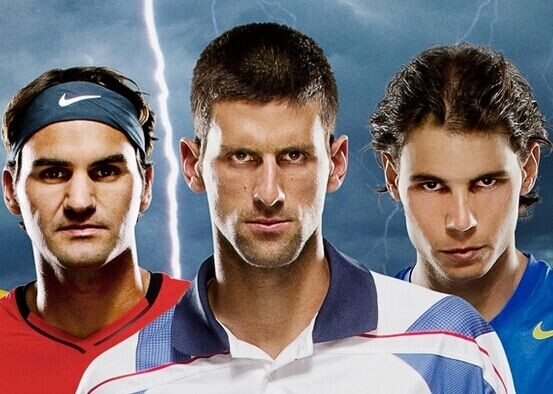
\includegraphics[width=0.6\textwidth]{img/FND.jpg}
        \caption{费德勒(左)、纳达尔(右)和德约科维奇(中)}
        \label{figure} % Put \label here!
    \end{figure}
    \section{数学公式}
    \subsection{公式}
    把行内公式 $E=mc^1$ 写成独立公式:
    \begin{equation*}
        E=mc^1.
    \end{equation*}

    把行内公式 $E=mc^2$ 写成有编号的独立公式:
    \begin{equation}
        E=mc^2. \label{eq2}
    \end{equation}

    把行内公式 $E=mc^3$ 写成有特殊编号的独立公式:
    \begin{equation}
        E=mc^3. \tag{$\ast$} \label{eq3}
    \end{equation}

    式~\eqref{eq2} 显然是对的. 式~\eqref{eq3} 连量纲都不对\dots{}
    \subsection{文字}
    这样写是错的:
    \begin{equation*}
        x > 0    任意 x \in R_+.
    \end{equation*}

    这样写才是对的:
    \begin{equation*}
        x > 0 \qquad \text{任意} \; x \in \mathbb{R_+}.
    \end{equation*}
    \subsection{上下标}
    \begin{equation*}
        \sum_{i=1}^{100} i = \sum^{100}_{j=1} j.
    \end{equation*}
    \begin{equation*}
        a^x+y \neq a^{x+y}.
    \end{equation*}
    \begin{equation*}
        e^{x^2} \neq {e^x}^2.
    \end{equation*}
    \subsection{根号}
    \begin{equation*}
        \sqrt{5} > \sqrt[5]{5}.
    \end{equation*}
    \subsection{函数名}
    这样写是错的:
    $ 2 \text{lim}_{x \rightarrow \infty} \text{arctan} x = \pi $.

    这样写才是对的:
    $ 2 \lim_{x \rightarrow \infty} \arctan x = \pi $.
    \subsection{模函数}
    \begin{equation*}
        5 \bmod 2 = 1.
    \end{equation*}
    \begin{equation*}
        5 \equiv 1 \pmod{2}.
    \end{equation*}
    \subsection{分数}
    \begin{equation*}
        \frac{\mathrm{d}^{n}y}{\mathrm{d}x^{n}}.
    \end{equation*}
    \begin{equation*}
        \frac{\partial^{2}z}{\partial{x}\partial{y}}.
    \end{equation*}
    \subsection{二项式系数}
    \begin{equation*}
        \binom{n}{k} = \binom{n-1}{k} + \binom{n-1}{k-1}.
    \end{equation*}
    \subsection{符号堆叠}
    $ 2\text{K}\text{Mn}\text{O}_4 \stackrel{\triangle}{\longrightarrow}
      \text{K}_2\text{Mn}\text{O}_4+\text{Mn}\text{O}_2+\text{O}_2\uparrow $,
    $ 2\text{H}_2\text{O}_2 \xrightarrow[]{\text{Mn}\text{O}_2}
    2\text{H}_2\text{O}+\text{O}_2\uparrow $.

    第二个更好!

    数学比化学复杂多了:
    \begin{equation*}
        \sum_{\substack{1\le{i}\le{n}\\j>i}} l_{ij}^2 = 0.
    \end{equation*}
    \subsection{矩阵}
    \begin{equation*}
        \boldsymbol{I} =
        \begin{bmatrix}
            1 & 0 \\
            0 & 1
        \end{bmatrix}.
    \end{equation*}
    \subsection{分段函数}
    \begin{equation*}
        |x| =
        \begin{cases}
            -x & \text{若} \  x < 0, \\
             0 & \text{若} \  x = 0, \\
             x & \text{若} \  x > 0. \\
        \end{cases}
    \end{equation*}
    \subsection{连等式}
    \begin{align}
        \nabla\frac{1}{r} & = \nabla\frac{1}{\sqrt{x^2+y^2+z^2}} \label{oeq}\\
            & = -\frac{x\boldsymbol{i}+y\boldsymbol{j}+z\boldsymbol{k}}
                      {\sqrt{x^2+y^2+z^2}^3} \nonumber \\
            & = -\frac{\hat{\boldsymbol{r}}}{r^2}. \tag{$\star$} \label{beq}
    \end{align}

    \eqref{oeq} 能直接从定义得出. 最后的结果 \eqref{beq} 非常漂亮!
    \subsection{空格}
    $ \text{这是} \  \text{1 space.} $

    $ \text{这是} \! \text{-3/18 em.} $

    $ \text{这是} \, \text{3/18 em.} $

    $ \text{这是} \: \text{4/18 em.} $

    $ \text{这是} \; \text{5/18 em.} $

    $ \text{这是} \quad \text{1 em.} $

    $ \text{这是} \qquad \text{2 em.} $
    \subsection{空位}
    这样写是错的: ${}^{99}_{ 9}\text{C}R_{abc}^{   d}$.

    这样写还是错的: ${}^{99}_{\ 9}\text{C}R_{abc}^{\ \ \ d}$.

    这样写才是对的: ${}^{99}_{\phantom{9}9}\text{C}R_{abc}^{\phantom{abc}d}$.
    \subsection{集合}
    这样写是错的: $\{\omega|X(\omega)\in\mathcal{B}\}$.

    这样写还是错的: $\{\omega\,|\,X(\omega)\in\mathcal{B}\}$.

    这样写才是对的: $\{\omega\mid X(\omega)\in\mathcal{B}\}$.
    \subsection{符号小全}
    这里解决不了的, \href{
        https://www.ctan.org/tex-archive/info/symbols/comprehensive
    }{究极符号大全}来解决!
    \begin{table}[!htbp]
        \centering
        \begin{tabular}{cccccc}
            $\dot{a}$ & \verb|\dot{a}| &
            $\bar{a}$ & \verb|\bar{a}| &
            $\hat{a}$ & \verb|\hat{a}| \\
            $\ddot{a}$ & \verb|\ddot{a}| &
            $\vec{a}$ & \verb|\vec{a}| \\
        \end{tabular}
    \end{table}
    \begin{table}[!htbp]
        \centering
        \begin{tabular}{cccccc}
            $<$ & \verb|<| &
            $>$ & \verb|>| &
            $=$ & \verb|=| \\
            $\leq$ & \verb|\leq| &
            $\geq$ & \verb|\geq| &
            $\equiv$ & \verb|\equiv| \\
            $\ll$ & \verb|\ll| &
            $\gg$ & \verb|\gg| \\
            $\in$ & \verb|\in| &
            $\ni$ & \verb|\ni| &
            $\sim$ & \verb|\sim| \\
            $\subset$ & \verb|\subset| &
            $\supset$ & \verb|\supset| &
            $\simeq$ & \verb|\simeq| \\
            $\subseteq$ & \verb|\subseteq| &
            $\supseteq$ & \verb|\supseteq| &
            $\approx$ & \verb|\approx| \\
            $:$ & \verb|:| &
            $\mid$ & \verb|\mid| &
            $\propto$ & \verb|\propto| \\
            $\perp$ & \verb|\perp| &
            $\parallel$ & \verb|\parallel| \\
            $\not\in$ & \verb|\not\in| &
            $\not\ni$ & \verb|\not\ni| &
            $\neq$ & \verb|\neq| \\
            $\not\subset$ & \verb|\not\subset| &
            $\not\supset$ & \verb|\not\supset| &
            $\not\equiv$ & \verb|\not\equiv| \\
            $\not\subseteq$ & \verb|\not\subseteq| &
            $\not\supseteq$ & \verb|\not\supseteq| \\
        \end{tabular}
    \end{table}
    \begin{table}[!htbp]
        \centering
        \begin{tabular}{cccccccc}
            $+$ & \verb|+| &
            $-$ & \verb|-| &
            $\times$ & \verb|\times| &
            $\div$ & \verb|\div| \\
            $\pm$ & \verb|\pm| &
            $\mp$ & \verb|\mp| &
            $\cdot$ & \verb|\cdot| &
            $/$ & \verb|/| \\
            $\cup$ & \verb|\cup| &
            $\cap$ & \verb|\cap| &
            $\oplus$ & \verb|\oplus| &
            $\otimes$ & \verb|\otimes| \\
            $\star$ & \verb|\star| &
            $\ast$ & \verb|\ast| &
            $\dagger$ & \verb|\dagger| &
            $\ddagger$ & \verb|\ddagger| \\
        \end{tabular}
    \end{table}
    \begin{table}[!htbp]
        \centering
        \begin{tabular}{cccccccc}
            $\sum$ & \verb|\sum| &
            $\prod$ & \verb|\prod| &
            $\bigcup$ & \verb|\bigcup| &
            $\bigcap$ & \verb|\bigcap| \\
            $\int$ & \verb|\int| &
            $\oint$ & \verb|\oint| &
            $\bigoplus$ & \verb|\bigoplus| &
            $\bigotimes$ & \verb|\bigotimes| \\
        \end{tabular}
    \end{table}
    \begin{table}[!htbp]
        \centering
        \begin{tabular}{cccc}
            $\leftarrow$ & \verb|\leftarrow| &
            $\longleftarrow$ & \verb|\longleftarrow| \\
            $\rightarrow$ & \verb|\rightarrow| &
            $\longrightarrow$ & \verb|\longrightarrow| \\
            $\leftrightarrow$ & \verb|\leftrightarrow| &
            $\longleftrightarrow$ & \verb|\longleftrightarrow| \\
            $\Leftarrow$ & \verb|\Leftarrow| &
            $\Longleftarrow$ & \verb|\Longleftarrow| \\
            $\Rightarrow$ & \verb|\Rightarrow| &
            $\Longrightarrow$ & \verb|\Longrightarrow| \\
            $\Leftrightarrow$ & \verb|\Leftrightarrow| &
            $\Longleftrightarrow$ & \verb|\Longleftrightarrow| \\
            $\mapsto$ & \verb|\mapsto| &
            $\longmapsto$ & \verb|\longmapsto| \\
            $\uparrow$ & \verb|\uparrow| &
            $\downarrow$ & \verb|\downarrow| \\
        \end{tabular}
    \end{table}
    \begin{table}[!htbp]
        \centering
        \begin{tabular}{cccc}
            $\overleftarrow{AB}$ & \verb|\overleftarrow{AB}| &
            $\underleftarrow{AB}$ & \verb|\underleftarrow{AB}| \\
            $\overrightarrow{AB}$ & \verb|\overrightarrow{AB}| &
            $\underrightarrow{AB}$ & \verb|\underrightarrow{AB}| \\
            $\overleftrightarrow{AB}$ & \verb|\overleftrightarrow{AB}| &
            $\underleftrightarrow{AB}$ & \verb|\underleftrightarrow{AB}| \\
        \end{tabular}
    \end{table}
    \begin{table}[!htbp]
        \centering
        \begin{tabular}{cccc}
            $(a)$ & \verb|(a)| &
            $[a]$ & \verb|[a]| \\
            $\{a\}$ & \verb|\{a\}| &
            $\langle{a}\rangle$ & \verb|\langle{a}\rangle| \\
            $\lfloor{a}\rfloor$ & \verb|\lfloor{a}\rfloor| &
            $\lceil{a}\rceil$ & \verb|\lceil{a}\rceil| \\
            $\lvert{a}\rvert$ & \verb|\lvert{a}\rvert| &
            $\lVert{a}\rVert$ & \verb|\lVert{a}\rVert| \\
        \end{tabular}
    \end{table}
    \begin{table}[!htbp]
        \centering
        \begin{tabular}{cccccccc}
            $\ldots$ & \verb|\ldots| &
            $\cdots$ & \verb|\cdots| &
            $\vdots$ & \verb|\vdots| &
            $\ddots$ & \verb|\ddots| \\
            $\because$ & \verb|\because| &
            $\therefore$ & \verb|\therefore| &
            $\infty$ & \verb|\infty| &
            $\%$ & \verb|\%| \\
            $\nabla$ & \verb|\nebla| &
            $\angle$ & \verb|\angle| &
            $\square$ & \verb|\square| &
            $\varnothing$ & \verb|\varnothing| \\
            $\hbar$ & \verb|\hbar| &
            $\ell$ & \verb|\ell| &
            $\Re$ & \verb|\Re| &
            $\Im$ & \verb|\Im| \\
            $\forall$ & \verb|\forall| &
            $\exists$ & \verb|\exists| &
            $\aleph$ & \verb|\aleph| &
            $\partial$ & \verb|\partial| \\
            $\S$ & \verb|\S| &
            $\P$ & \verb|\P| \\
        \end{tabular}
    \end{table}
    \newpage
    \section{参考文献}
    % 这里用的是 BibTeX.
    % 也可尝试 natbib 和 biblatex.
    FRBs are millisecond-duration bright radio transients
    \cite{Li2018,Lin2020}.
    \bibliographystyle{abbrv}
    \bibliography{astro}
    \section{自定义命令}
    \def\lshortURL{https://www.ctan.org/pkg/lshort}
    \def\lnotesURL{https://github.com/huangxg/lnotes}
    \newcommand{\isgood}[3][是好的]{\href{#3}{#2} #1!}

    \isgood{lshort}{\lshortURL}

    \isgood[也是好的]{lnotes}{\lnotesURL}
    \section{超链接}
    想让\href{clexample.pdf}{《\LaTeX{}范例集》}变得更好?

    可以在 \href{https://github.com/GasinAn/lexamples}{Github}
    上提交 pull request 或 issue.

    也可以发邮件至 \href{mailto:gasin185@163.com}{gasin185@163.com}.
\end{document}
